\documentclass[spanish,notitlepage,letterpaper, 12pt]{article}
\usepackage[spanish]{babel} 
\usepackage{amsmath}
\usepackage{amsfonts}
\usepackage{amssymb}
\usepackage{graphicx}
\usepackage{geometry}      
\geometry{letterpaper}                  
\usepackage{epstopdf}
\usepackage{fancyhdr} % Paquete para encabezados y pies de pag
\usepackage{color}
\usepackage{placeins}
\usepackage{csquotes}
\usepackage{textcomp}
\usepackage{gensymb}
\usepackage{array}
\usepackage{pgfplots}
\usepackage{circuitikz}
\usepackage{tikz}

%Specifies how thick the bipoles are, e.g. the capacitor, the inductor, ...
\ctikzset{bipoles/thickness=1.2}

\pagestyle{fancy}
\chead{\bfseries Informe 4 - Grupo C1B. Subgrupo 2} 
\rhead{1 de Junio de 2023}
\cfoot{Universidad Industrial de Santander} 
\rfoot{\thepage} 

\pgfplotsset{compat=1.18, width=10cm}
\voffset = -0.25in 
\textheight = 8.0in 
\textwidth = 6.5in
\oddsidemargin = 0.in
\headheight = 20pt 
\headwidth = 6.5in
\renewcommand{\headrulewidth}{0.5pt}
\renewcommand{\footrulewidth}{0,5pt}
\begin{document}
\begin{titlepage}
    \begin{center}
        
\includegraphics[width=0.4\textwidth]{../general-images/uis-logo.png}
        
        \vspace{0.5cm}
        \LARGE
        \textbf{Estudio del comportamiento del circuito RLC y el fenómeno de resonancia}
        
        \vspace{0.5cm}
        \large
        Informe 4
        
        \vfill
        
        \textbf{Daniel Esteban Vargas Reyes.} Estudiante - Geología\\
        \textbf{Nicolás Andrés Ramírez Calderón.} Estudiante - Ingeniería de Sistemas\\ 
        \textbf{Rodolfo Valentín Muñoz Vega.} Estudiante - Ingeniería Química\\

        \vspace{1.0cm}
        Presentado a la docente:
        
        \textbf{Zayda Paola Reyes Quijano}
        
        \vfill
        
        Escuela de Física - Física III\\
        Universidad Industrial de Santander\\
        Bucaramanga, Santander, Colombia\\
        20 de Mayo de 2023        
    \end{center}
\end{titlepage}

\tableofcontents

\newpage

\section{Resumen}
El siguiente laboratorio se desarrolla con la finalidad de aplicar los conocimientos en el tema de circuitos RLC, conociendo su comportamiento y capacidad a través de un multímetro, osciloscopio, una fuente de voltaje, dispositivo para establecer el valor de capacitancia, inductancia y resistencia. En donde se busca analizar experimentalmente la frecuencia de resonancia por medio del osciloscopio y hacer una comparación con la obtenida teóricamente. También se desea analizar el voltaje en la resistencia, la inductancia y la capacitancia bajo diferentes frecuencias incluyendo la de resonancia, así mismo, calcular el valor de impedancia para las diferentes frecuencias. Por medio de estos datos se entra en comparación con los teóricos para obtener un porcentaje de error entre ellos.
\section{Introducción}
Los circuitos eléctricos representan un eje fundamental en la sociedad actual. Aquellos de tipo RLC son alimentados por una
fuente AC de voltaje constante $V$ y frecuencia variable $\omega$ , la corriente que
aparece en este circuito tiene la misma frecuencia angular que la fuente y una
amplitud de la corriente $I = \frac{V}{Z}$ , donde $Z$ es la impedancia del circuito. Esta
impedancia está relacionada con la reactancia capacitiva $X_C$, la reactancia
inductiva $X_L$, y la resistencia. Una de las características principales que tienen
estas reactancias es su dependencia con la frecuencia de la fuente de
alimentación, lo que conduce a que la impedancia depende de $\omega$.\par
\subsection{Objetivos}
\begin{itemize}
    \item \textbf{General: }Estudiar las características de un circuito RLC en serie con una fuente de
alimentación alterna y el fenómeno de resonancia.
\item \textbf{Específicos: }
    \begin{enumerate}
        \item Determinar teórica y experimentalmente la frecuencia de resonancia de un circuito RLC.
        \item Estudiar el efecto sobre el voltaje en cada elemento del circuito RLC y la
corriente eficaz, por la variación de la frecuencia dada por la fuente de
voltaje AC.
        \item Estudiar cómo cambia la frecuencia de resonancia del circuito RLC con
la variación de la resistencia.
    \end{enumerate}
\end{itemize}
\subsection{Marco teórico} \label{I.MT}
\subsubsection{Oscilaciones en un circuito RLC}
Para entender la respuesta natural del circuito RLC de manera intuitiva, es pertinente pensar en el movimiento de la carga en el circuito a lo largo del tiempo.\par
\begin{figure}[!ht]
    \centering
    \begin{circuitikz}
        % Circuit
        \draw[line width=0.8]
        (2,7) to (2,1)
        (2,7) to [resistor, l_=$R$] ++(6,0) to [inductor, l_=$L$] ++(0,-6) to [capacitor, l_=$C$] +(-6,0) ;
        % Grid
        %\draw[help lines] (0,0) grid (10,10);
    \end{circuitikz}
    \caption{\textit{Circuito RLC.}}
    \label{fig:rlc}
\end{figure}
Si se coloca una carga inicial en el capacitor y después se cierra el interruptor (Fig. \ref{fig:rlc}), la carga irá de una placa del capacitor a la otra, pasando a través del
inductor y del resistor en ambas direcciones. Cada ciclo de oscilación será un poco menor que el anterior, porque se pierde energía conforme la carga en
movimiento calienta el resistor (Fig. \ref{fig:q-in-time}).\par
\begin{figure}[!ht]
    \centering
    \begin{tikzpicture}
        \begin{axis}
            [
            axis lines = center,
            domain = 0:3,
            xlabel = $t$,
            xmin = -0.5,
            xmax = 3.5,
            xtick={0},
            ylabel = $q$,
            ymin=-1.5,
            ymax=1.5,
            ytick={-1,1},
            yticklabels={$-q_{max}$,$q_{max}$},
            samples=50,
            ]
            \addplot [orange] {e^(-3*x/4)*cos(deg(2*pi*x))};
            \addplot [dashed] {e^(-3*x/4)}
                node[right,pos=0.2]{$q_{max}e^{-\frac{Rt}{2L}}$};
            \addplot [dashed] {-e^(-3*x/4)}
                node[right,pos=0.2]{$-q_{max}(-e^{-\frac{Rt}{2L}})$};
        \end{axis}
    \end{tikzpicture}
    \caption{\textit{Gráfica de la carga en función del tiempo para el capacitor en un circuito RLC.}}
    \label{fig:q-in-time}
\end{figure}
\newpage
Para el análisis que se pretende se puede escribir el cambio de energía como una función del tiempo. \cite{serway_jewett_2017}\par
\begin{equation}\label{eq:energy}
    \frac{du}{dt}=\frac{q}{c}\frac{dq}{dt}+iL\frac{di}{dt}=-i^{2}R
\end{equation}
Al reemplazar $i=\frac{dq}{dy}$ y $\frac{di}{dt}=\frac{d^qq}{dt^2}$ en \eqref{eq:energy} se tiene que:
\begin{equation}\label{eq:ed-rlc}
    \frac{d^2q}{dt^2}+\frac{R}{L}\frac{dq}{dt}+\frac{q}{LC}=0
\end{equation}
La solución de \eqref{eq:ed-rlc} es $q=q_{max}e^{-\frac{Rt}{2L}}\cos{(\omega t)}$ donde:
\begin{equation}\label{eq:frequency}
    \omega=\sqrt{\omega_0-\frac{R}{2L}^2}
\end{equation}
    Siendo $\omega_0=\frac{1}{\sqrt{LC}}$ la frecuencia angular de resonancia.
\subsubsection{Circuito RLC en serie}
La corriente que varía con el timepo en el circuito RLC puede describirse como el fasor $I_m$ sobre eleje vertical, donde el ángulo de dicho fasor es $(\omega t-\theta)$ tal y como se representa en \eqref{eq:i-fasor}.
\begin{equation}\label{eq:i-fasor}
    i=I_m\sin(\omega t-\theta)
\end{equation}
Donde $I_m$ es la magnitud del fasor $\vec{I_m}$. El voltaje a través de todos los componentes en el circuito está dado por la fuente $fem$ que varía con el tiempo. (Fig. \ref{fig:rlc-fem})\par
\bigskip
\begin{figure}[ht]
    \centering
    \begin{circuitikz}
        \draw[line width=0.8]
        (2,7) to [sinusoidal voltage source, l_=$V_S$, i=$I$] (2,1)
        (2,7) to [resistor, l_=$R$] ++(6,0) to [inductor, l_=$L$] ++(0,-6) to [capacitor, l_=$C$] +(-6,0) ;
        % Grid
        %\draw[help lines] (0,0) grid (10,10);
    \end{circuitikz}
    \caption{\textit{Circuito RLC con FEM variable en el tiempo.}}
    \label{fig:rlc-fem}
\end{figure}
La ecuación \eqref{eq:rlc-voltage} también representa el cambio de este voltaje\par
\begin{equation}\label{eq:rlc-voltage}
    V=V_{fem}(t)=V_m\sin{(\omega t)}
\end{equation}
\begin{figure}[!ht]
    \centering
    \begin{tikzpicture}[scale=1.5, transform shape]
        \draw[line width=0.8,dashed]
            (0,1.25) node[left] {$i$} to (2.150,1.25) ;

        \coordinate (vec1) at (0:1.5); 
        \coordinate (vec2) at (30:2.5);
        \coordinate (vec3) at (0:2.5);
        \coordinate (vec4) at (90:2);
        \coordinate (vec5) at (270:2);
        \coordinate (vec6) at (180:2);

        \draw[->,thick,green] (0,0) -- (vec2) node[below right, black] {$I_m$};
        \draw[->,thick,black] (0,0) -- (vec3);
        \draw[->,thick,black] (0,0) -- (vec4);
        \draw[->,thick,black] (0,0) -- (vec5);
        \draw[->,thick,black] (0,0) -- (vec6);

        \draw [thick] (1.0,0) arc (0:30:1cm)    node [midway, right] {$\omega t-\theta$};
        % Grid
        %\draw[help lines] (-3,-3) grid (3,3);
    \end{tikzpicture}
    \caption{\textit{Fasor de corriente.}}
    \label{fig:current-fasor}
\end{figure}
\newpage
En este circuito, el resistor, el voltae $V_R$ y la corriente $i$ están en fase entre sí. Mientras que el fasor voltaje $V_m$ está en fase con $I_m$ (Fig. \ref{fig:current-fasor}). La corriente $i$ está adelante del voltaje $V_c$, de modo que dicho fasor tiene un ángulo que es menor del de $I_m$ y $V_R$. La corriente del inductor
$i$ se atrasa con respecto al voltaje $V_L$ por $\frac{\pi}{2}\ rad$ más que los ángulos de $I_m$ y $V_R$. (Fig. \ref{fig:voltage-fasor})
\begin{figure}[!ht]
    \centering
    \begin{tikzpicture}

        \coordinate (vec1) at (120:2.5); 
        \coordinate (vec2) at (30:2.5);
        \coordinate (vec3) at (-60:2.5);
        \coordinate (vec4) at (0:3);
        \coordinate (vec5) at (90:3);
        \coordinate (vec6) at (270:3);
        \coordinate (vec7) at (180:3);

        \draw[line width=0.8,dashed] (0,1.25) node[left] {$V_R$} -- (vec2);
        \draw[line width=0.8,dashed] (0,2.165) node[right] {$V_L$} -- (vec1);
        \draw[line width=0.8,dashed] (0,-2.165) node[left] {$V_C$} -- (vec3);

        \draw[->,thick,red] (0,0) -- (vec1) node[below left, black] {$\vec{V_L}$};
        \draw[->,thick,red] (0,0) -- (vec2) node[below right, black] {$\vec{V_R}$};
        \draw[->,thick,red] (0,0) -- (vec3) node[above right, black] {$\vec{V_C}$};
        \draw[->,thick,black] (0,0) -- (vec4);
        \draw[->,thick,black] (0,0) -- (vec5);
        \draw[->,thick,black] (0,0) -- (vec6);
        \draw[->,thick,black] (0,0) -- (vec7);

        \draw [thick] (1.0,0) arc (0:30:1cm) node [midway, right] {$\omega t-\theta$};
        % Grid
        %\draw[help lines] (-3,-3) grid (3,3);
    \end{tikzpicture}
    \caption{\textit{Fasor de voltajes.}}
    \label{fig:voltage-fasor}
\end{figure}
\subsubsection{Impedancia}
La impedancia de un circuito depende de la frecuencia de la $fem$ , se denota con
el símbolo $Z$ y tiene la unidad de ohm, justo como la resistencia.
\begin{equation}\label{eq:impedance}
    Z=\sqrt{R^2+(X_L-X_C)^2}
\end{equation}
La corriente que circula en un circuito de CA depende de la diferencia entre la reactancia inductiva $R_L$ y la capacitiva $R_A$ y se denomina \textbf{reactancia total}. La ecuación \eqref{eq:impedance} ilustra esta diferencia.\par
\bigskip
Para un circuito RLC conectado en serie existen tres situaciones:
\begin{enumerate}
    \item Si $X_L>X_C$\\
        $\theta$ es positivo y la corriente en el circuito va detras del voltaje en el circuito (se asemeja a uno con un solo inductor).
    \item Si $X_L<X_C$\\
        $\theta$ es negativo y la corriente en el circuito va adelante del voltaje en el circuito (parece uno con un solo capacitor) 
    \item Si $X_L=X_C$\\
        $\theta$ es cero y la corriente en el circuito se encontrará en fase con el voltaje del mismo, luego se asemeja a un circuito con una sola resistencia. Cuando $\theta=0$ se dice que el circuito está en resonancia.
\end{enumerate}
La amplitud de la corriente $I_m$ en el circuito RCL en serie depende de la frecuencia de la $fem$ que varía con el tiempo y se produce cuando el sistema está en resonancia.
\begin{equation}
    \omega L=\frac{1}{\omega C}=0
\end{equation}
La energía que almacenan temporalmente los campos se devuelve al circuito (por ejemplo cuando el capacitor se descarga o el campo magnético del
inductor se autoinduce). Esto hace que la potencia total suministrada por la
fuente no siempre sea la consumida por el circuito. Parte de la potencia se utiliza para crear estos campos, pero no se consume. Sin embargo, la fuente debe proveerla para el funcionamiento del circuito.
\subsubsection{Potencia reactiva}
Se trata de la potencia necesaria para crear los campos eléctricos y magnéticos. Es una
potencia devuelta por el circuito, pero que está presente en el funcionamiento.
Se mide en watts.
\begin{equation}
    Q=I^2\cdot(X_L-X_C)
\end{equation}
Los medidores de voltaje y corriente utilizados miden los valores eficaces o valores rms (root mean square).
\begin{equation}
    V_{ef}=\frac{V_{max}}{\sqrt{2}}
\end{equation}
\begin{equation}
    I_{ef}=\frac{I_{max}}{\sqrt{2}}
\end{equation}
\section{Metodología}
Para desarrollar esta práctica de laboratorio se plantean dow fases
metodológicas. En la primera fase se midió y estudió el fenómeno de
resonancia en el circuito RLC, en la segunda fase se tomaron mediciones de
voltaje y corriente sobre los elementos RLC para diferentes frecuencias.
\subsection{Materiales}
\begin{enumerate}
    \item Osciloscopio.
    \item Fuente de alimentación de voltaje.
    \item Dispositivo de capacitancia.
    \item Dispositivo de reactancia.
    \item Dispositivo de resistencia.
    \item Multímetro.
\end{enumerate}
\subsection{Fase 1} \label{M.F1}
Se ubicó el inductor, condensador y una resistencia en serie, luego se alimentó el circuito con una fuente de voltaje constante
$V$ y frecuencia variable $\omega$.\par
\bigskip
En esta primera parte se determinó la frecuencia de resonancia de todo el circuito. Primero se realizó el cálculo teórico haciendo uso de la ecuación \eqref{eq:frequency}.
Posteriormente se colocó un valor de voltaje en el circuito y se seleccionó el
valor de frecuencia de resonancia hallado teóricamente. Para comprobar que
este era el valor experimental de la frecuencia de resonancia, se midió el
voltaje en cada uno de los elementos con ayuda del voltímetro.\par 
\bigskip
Al realizar las
mediciones, el voltaje presentó un valor máximo cuando el valor del
voltaje del capacitor y el inductor eran iguales. Además el valor de la corriente
era máxima comparada con la medición en otro valor diferente a la
frecuencia de resonancia. Sin embargo, para el valor calculado el sistema no
estaba en resonancia, así que fue necesario ajustar con la perrilla el valor de frecuencia que hace que el
sistema alcanzara esta condición.
\subsection{Fase 2} \label{M.F2}
Una vez hallado el valor experimental de la frecuencia de Resonancia,
ahora se estudió la variación del voltaje en cada elemento del circuito y la
corriente, para esto fue preciso cambiar la frecuencia de la fuente AC. Se probaron valores
por debajo y por encima del valor de frecuencia de resonancia calculado para la
fase anterior. Para cada valor de frecuencia, se registraron, los voltajes sobre la resistencia, el capacitor y el inductor y la corriente del circuito.\par 
\bigskip
Para estudiar la
dependencia de la impedancia $Z$ con $\omega$ , se empleó la ecuación \eqref{eq:impedance}, primero se determinaron
los valores teóricos de $X_L$ , $X_C$ y se halló $Z$. Posteriormente se determinaron los valores
experimentales de $X_L$ , $X_C$ y $Z$, usando los valores de voltajes y corriente
medidos. También se comparó el valor de $Z$ teórico y experimental y se estudió su
comportamiento con la frecuencia $\omega$.
\section{Tratamiento de datos} \label{TD}
\subsection{Primera parte}
Se tomaron los datos de resistencia, inductancia y capacitancia, para calcular la frecuencia de resonancia teórica a partir de estos datos. (Cdr. \ref{tab:rlc})\par
\begin{table}[ht]
    \centering
    \begin{tabular}{|c|c|c|c|c|c|c|}
        \hline
        $R\ [\ohm]$ & $L\ [mH]$ & $C\ [\mu F]$ & $F_{\text{resonancia}}\ [Hz]$ & $V_R\ [V]$ & $V_L\ [V]$ & $V_C\ [V]$ \\
        \hline\hline
        $10$ & $17$ & $10$ & $386.007$ & $1.44$ & $6.45$ & $6.47$\\
        $100$ & $4$ & $1$ & $2516.46$ & $5.04$ & $3.54$ & $3.57$\\
        $230$ & $4$ & $1$ & $2516.46$ & $5.75$ & $166$ & $1.66$\\
        \hline
    \end{tabular}
    \caption{\textit{Voltajes medidos para diferentes valores de $R$, $L$ y $C$. Frecuencia de resonancia teórica.}}
    \label{tab:rlc}
\end{table}
La frecuencia teórica fue encontrada a partir de su fórmula \eqref{eq:frequency}. A continuación se contrastan los valores teóricos con los experimentales (Cdr. \ref{tab:frequ}) a la vez que se calcula el porcentaje de error \eqref{eq:error}.\par
\begin{equation}\label{eq:error}
    \text{\% error}=\frac{F_{\text{teórica}}-F_{\text{experimental}}}{F_{\text{teórica}}}\times100\%
\end{equation}
\begin{table}[ht]
    \centering
    \begin{tabular}{|c|c|c|}
        \hline
        $F_{\text{teórica}}$ & $F_{\text{experimental}}$ & \% error\\
        \hline\hline
        $386.007$ & $305.2$ & $20\%$\\
        $2516.46$ & $2517$ & $0.02\%$\\
        $2516.46$ & $2464$ & $2\%$\\
        \hline
    \end{tabular}
    \caption{\textit{Porcentajes de error de las frecuencias obtenidas.}}
    \label{tab:frequ}
\end{table}
\subsection{Segunda parte}
De la tabla para la que se toman datos con diferentes frecencias (Cdr. \ref{tab:var-freq}) se puede observar que al acercarse la frecuencia en el circuito RLC la amplitud aumenta y el dicho circuito entra en resonancia. Además, al realizar la toma de datos se comprobó dicha frecuencia tanto
experimental como teóricamente, asumiendo que el voltaje en la inductancia y la capacitancia son casi iguales o tienen valores muy cercanos, es así que lo evidenciamos en el porcentaje de error de dichas frecuencias, este valor se puede llegar a presentar debido a errores en la toma de datos o
calibración de los equipos del laboratorio.\par
\begin{table}[ht]
    \centering
    \begin{tabular}{|c|c|c|c|c|c|c|}
        \hline
        $f\ [Hz]$ & $V_R\ [V]$ & $V_I\ [V]$ & $V_C\ [V]$ & $I_{exp}\ A$ & $P_{exp}\ [W]$ & $Z_{exp}$\\
        \hline\hline
        $1604$ & $5.83$ & $2.53$ & $1.15$ & $0.0252$ & $0.146916$ & $5.9911$\\
        $1799$ & $5.87$ & $2.25$ & $1.22$ & $0.0254$ & $0.149098$ & $5.9596$\\
        $2024$ & $5.81$ & $1.97$ & $1.38$ & $0.0252$ & $0.146410$ & $5.9399$\\
        $2273$ & $5.78$ & $1.72$ & $1.52$ & $0.0255$ & $0.147390$ & $5.7835$\\
        $2490$ & $5.61$ & $1.51$ & $1.64$ & $0.0249$ & $0.139690$ & $5.6115$\\
        $2698$ & $5.61$ & $1.37$ & $1.76$ & $0.0250$ & $0.140250$ & $5.6235$\\
        $1799$ & $5.57$ & $1.23$ & $1.86$ & $0.0250$ & $0.139250$ & $5.6055$\\
        $1799$ & $5.54$ & $1.15$ & $1.94$ & $0.0253$ & $0.140160$ & $5.5960$\\
        $1799$ & $5.50$ & $1.07$ & $1.04$ & $0.0253$ & $0.139150$ & $5.5849$\\
        \hline
    \end{tabular}
    \caption{\textit{Valores para distintas frecuencias del circuito RLC.}}
    \label{tab:var-freq}
\end{table}
A continuación se presenta una gráfica que ilustra el comportamiento de los voltajes en el capacitor y en el inductor a medida que cambia la frecuencia. (Fig. \ref{fig:voltages-vs-freq})\par
\begin{figure}[ht]
    \centering
    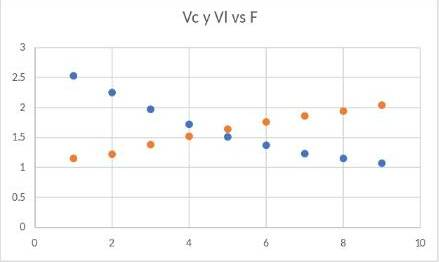
\includegraphics[width=10cm]{images/capacitor-vs-inductor-voltages.jpg}
    \caption{\textit{Voltajes de capacitor e inductor vs frecuencia.}}
    \label{fig:voltages-vs-freq}
\end{figure}
Por otra parte, también se ilustran las gráficas que representan el cambio en el voltaje de la resistencia (Fig. \ref{fig:voltage-r-vs-freq}) así como el cambio de la corriente en el circuito (Fig. \ref{fig:current-vs-freq}).\par
\newpage
\begin{figure}[ht]
    \centering
    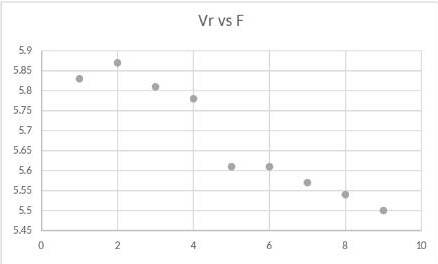
\includegraphics[width=10cm]{images/resistor-voltage.jpg}
    \caption{\textit{Voltajes de resistor vs frecuencia.}}
    \label{fig:voltage-r-vs-freq}
\end{figure}
\begin{figure}[ht]
    \centering
    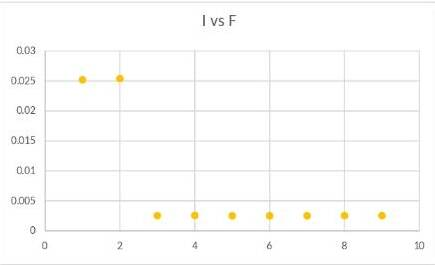
\includegraphics[width=10cm]{images/current.jpg}
    \caption{\textit{Corriente vs frecuencia.}}
    \label{fig:current-vs-freq}
\end{figure}
\section{Análisis de resultados}
La parte analítica y comprensiva de este laboratorio fue fundamental para su desarrollo, se llevaron a cabo varias mediciones para obtener los respectivos datos de resistencia, inductancia y capacitancia para calcular una frecuencia de resonancia teórica con dichos datos, esto se hizo con las formulas señaladas en el tratamiento de datos, en respuesta al uso de estas fórmulas se obtuvieron datos que se compararían con su contraparte experimental, siendo que en la primera parte hubo un porcentaje de error muy bajo, y se podría decir que despreciable, más sin embargo existente, que se pueden presentar debido a errores en la toma de datos o en la calibración de los equipos de laboratorio, por otra parte se comprobó que al aumentar la frecuencia del circuito RLC, la intensidad aumenta y el circuito entra en resonancia.
\section{Conclusiones}
Cerrando con el proceso de experimentación, toma de datos y análisis de estos mismos, se puede decir que se cumplieron los objetivos propuestos al inicio de dicho laboratorio, como parte principal para el entendimiento de cómo funciona un circuido RLC en función de la frecuencia, y al cambiar valores de resistencia, inductancia y capacitancia, tambien se halló de manera satisfactorio cuando el circuito RLC, se encuentra en resonancia.
\section{Referencias} 
\bibliographystyle{unsrt}
\bibliography{../general-references/references}
\end{document}
